\documentclass{beamer}[10]
\usetheme{default}
\usepackage{pgf}
\usepackage[utf8]{inputenc}
\usepackage[brazil]{babel}
\usepackage{beamerthemesplit}
\usepackage{graphics,epsfig, subfigure}
\usepackage{url}
\usepackage{srcltx}
\usepackage{hyperref}



\title[Cobertura Mínima de Vértices]
{\textbf{Uma Heurística para o Problema da Cobertura Mínima de
    Vértices}}
\author[guedesav, dggc]{Bruno Guedes, Daniel Galinkin}

\institute[UFMG] % opcional
{Departamento de Ciência da Computação
\\Universidade Federal de Minas Gerais}

\subject{Teoria de Grafos}

\date{\today}

\begin{document}

   \frame{\titlepage}

   % Mostra um table of contents no inicio de cada subsection:
   \AtBeginSection[] {
     \begin{frame}<beamer>{Sumário}
       \tableofcontents[currentsection,currentsubsection]
     \end{frame}
   }
   \AtBeginSubsection[] {
     \begin{frame}<beamer>{Sumário}
       \tableofcontents[currentsection,currentsubsection]
     \end{frame}
   }

    
\section{Introdução}
\subsection{Definição}
    
\frame{
\frametitle{Definição}
Dado um grafo $G = (V, E)$, uma cobertura de vértices (\textit{CV}) é
    um subconjunto $C \subseteq V \mid \forall e=(a,b) \in E, a \in C
    \mbox{ ou } b \in C$.

O problema da cobertura mínima de vértices (\textit{CMV}) consiste em
encontrar $C^*$ tal que, seja $K$ o conjunto das coberturas de
vértices de $G$, $\left| C^* \right| \leq \left| C \right| \forall C
\in K$.

\begin{figure}[htb]
\centering
\subfigure[Coberturas não mínimas de vértices]{
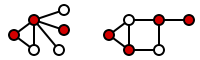
\includegraphics[width=0.4\textwidth]{../doc/img/vertex-cover.png}
\label{fig:cv}
}
\subfigure[Coberturas mínimas de vértices]{
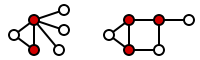
\includegraphics[width=0.4\textwidth]{../doc/img/minimum-vertex-cover.png}
\label{fig:cmv}
}
\caption{Exemplos de coberturas de vértices}
\label{fig:cv-cmv}
\end{figure}
}


\subsection{Aplicações}
\frame{
\frametitle{Definição}
\begin{itemize}
    \item Vários algoritmos em bioinformática, como encontrar árvores
        filogenéticas, identificação de fenótipos e análise de dados
        de microarranjos.
    \item Clustering em redes sem fios.
\end{itemize}
}

\subsection{Complexidade}
\frame{
\frametitle{Complexidade}
\begin{itemize}
\item Para o caso geral, encontrar a CMV de um grafo $G = (V, E)$ é um
    problema NP-Completo.

\item Um algoritmo que encontre a CMV $C$ por busca exaustiva executa
em tempo $2^{O(k)n^{O(1)}}$, onde $n = \left| V \right|$ e $k = \left|
C \right|$.

\item Utilizando a técnica de \textit{bounded search
tree algorithm}, é possível reduzir o tempo de execução para
$2^{o(k)n^{O(1)}}$.
\end{itemize}
}

\section{Algoritmos conhecidos}
\subsection{Algoritmos aproximativos}
\frame{
\frametitle{Primeiro algoritmo}
\begin{block}{primeiroAlgoritmo($G$)}
\begin{enumerate}
    \item $C \rightarrow \emptyset$
    \item while $E \ne \emptyset$
    \begin{enumerate}
        \item Escolha $e = (a,b) \in E$ aribitrariamente.
        \item $C = C \cup \{a,b\}$
        \item $E \rightarrow E \backslash \{e \in E : a \mbox{ ou } b
        \in e\}$
    \end{enumerate}
\end{enumerate}
\end{block}

\begin{itemize}
    \item Sempre acha uma solução até 2 vezes pior que a solução
        ótima.
    \item Executa em $O(V+E)$.
    \item Descoberto independentemente por~\cite{cite:simple}.
\end{itemize}
}

\frame{
\frametitle{Segundo algoritmo}
\begin{itemize}
    \item Existem algoritmos com um fator de aproximação ligeiramente
        melhores.
    \item Um algoritmo, usando técnicas avançadas e programação
    linear, é conhecido~\cite{cite:complex}. Seu fator de aproximação
    é de $2 - \Theta(\dfrac{1}{\sqrt{\log V}})$, e é o melhor fator
    encontrado na literatura.
\end{itemize}
}

\subsection{Heurísticas}
\frame[allowframebreaks]{
\frametitle{Algoritmo guloso}
\begin{block}{Guloso($G$)}
\begin{enumerate}
    \item $C \rightarrow \emptyset$
    \item while $E \ne \emptyset$
    \begin{enumerate}
        \item Seja $v \in G : d[v] \ge d[u], \forall u \in V$
        \item $C = C \cup \{v\}$
        \item $E \rightarrow E \backslash \{e \in E : v \in e\}$
    \end{enumerate}
\end{enumerate}
\end{block}

O algoritmo acima parte do príncipio de escolher os vértices que têm
mais arestas incidentes a ele para o CMV, de forma a cobrir o mais
número de arestas com o menor número de vértices.

\framebreak

No entanto, este algoritmo falha mais vezes que a intuição indica.

\begin{figure}[htb]
\centering
\subfigure[Caso ótimo]{
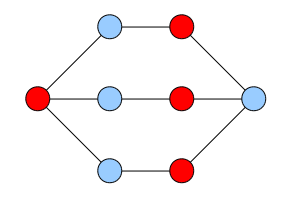
\includegraphics[width=0.4\textwidth]{../doc/img/optimal.png}
\label{fig:optimalguloso}
}
\subfigure[Solução encontrada]{
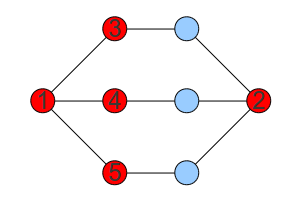
\includegraphics[width=0.4\textwidth]{../doc/img/wrong.png}
\label{fig:wrongguloso}
}
\caption{Exemplo de caso em que o algoritmo guloso falha}
\label{fig:guloso}
\end{figure}
}

\section{Heurística proposta}
\subsection{Príncipio}
\frame{
\frametitle{Príncipio}

\begin{block}{Princípio}
Se existe uma aresta $e=(u,v)$, e $d[u] = 1$,
então existe uma CMV $C$ tal que $v \in C$.
\end{block}

\begin{figure}[htb]
\centering
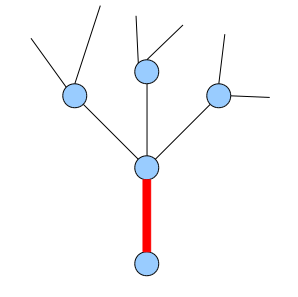
\includegraphics[width=0.3\textwidth]{../doc/img/principio.png}
\caption{Exemplo de escolha ótima local}
\label{fig:principio}
\end{figure}
}


\subsection{Pseudo-algoritmo}
\frame{
\frametitle{Pseudo-algoritmo}
\begin{block}{heuristica($G$)}
\begin{enumerate}
    \item $C \rightarrow \emptyset$
    \item while $E \ne \emptyset$
    \begin{enumerate}
        \item Se existe $u \in V : d[u] = 1$, faça $chosen = v :
            e=(u,v) \in E$.
        \item Senão, seja $v \in G : d[v] \ge d[u], \forall u \in V$.
        Faça $chosen = v$.
        \item $C = C \cup \{chosen\}$
        \item $E \rightarrow E \backslash \{e \in E : chosen \in e\}$
    \end{enumerate}
\end{enumerate}
\end{block}

\begin{itemize}
    \item Executa em $O(VE)$.
    \item O passo no item 2.2 é uma escolha gulosa, e
    passível de ser adaptada para alguma estratégia mais elaborada.
\end{itemize}
}


\subsection{Execução passo a passo}
\frame[allowframebreaks]{
\frametitle{Passo}

\begin{figure}[ht]
\centering
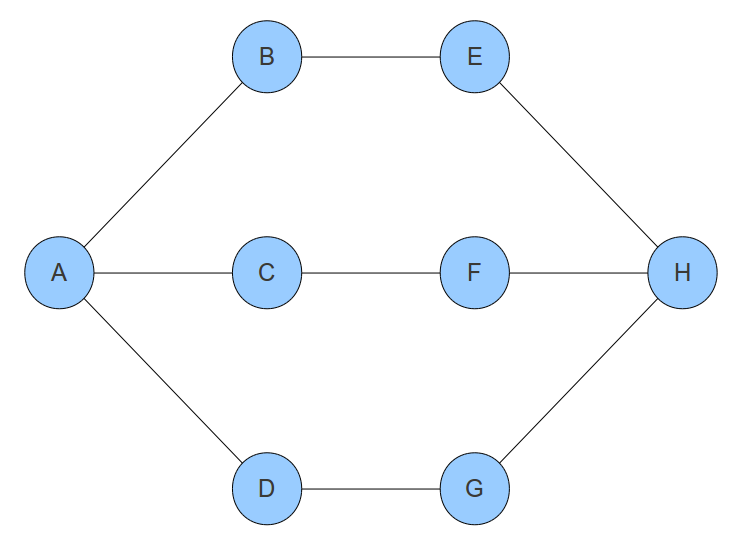
\includegraphics[width=0.5\textwidth]{../doc/img/exemplo1/passo1.png}
\caption{$C=\emptyset$}
\label{fig:exemplo1-passo1}
\end{figure}


\begin{figure}[ht]
\centering
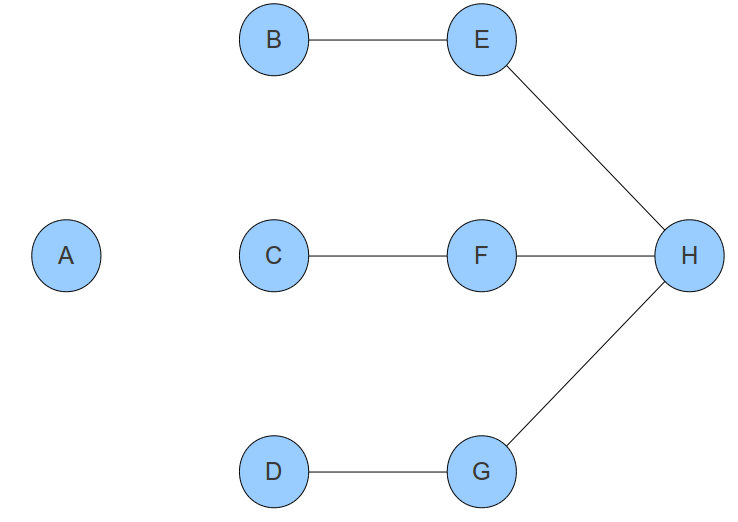
\includegraphics[width=0.5\textwidth]{../doc/img/exemplo1/passo2.png}
\caption{$C=\{A\}$}
\label{fig:exemplo1-passo2}
\end{figure}


\begin{figure}[ht]
\centering
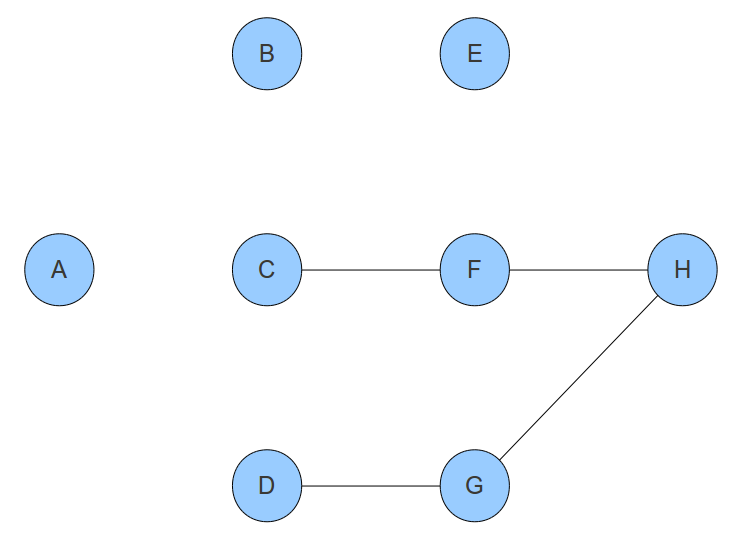
\includegraphics[width=0.5\textwidth]{../doc/img/exemplo1/passo3.png}
\caption{$C=\{A, E\}$}
\label{fig:exemplo1-passo3}
\end{figure}


\begin{figure}[ht]
\centering
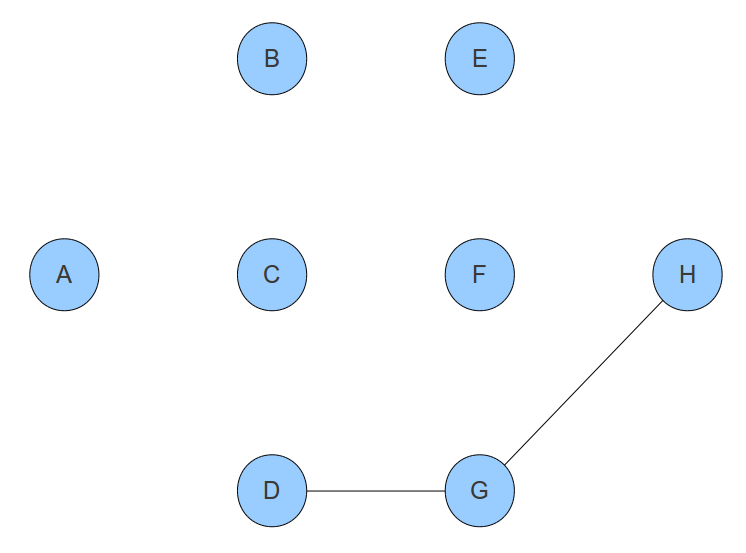
\includegraphics[width=0.5\textwidth]{../doc/img/exemplo1/passo4.png}
\caption{$C=\{A, E, F\}$}
\label{fig:exemplo1-passo4}
\end{figure}


\begin{figure}[ht]
\centering
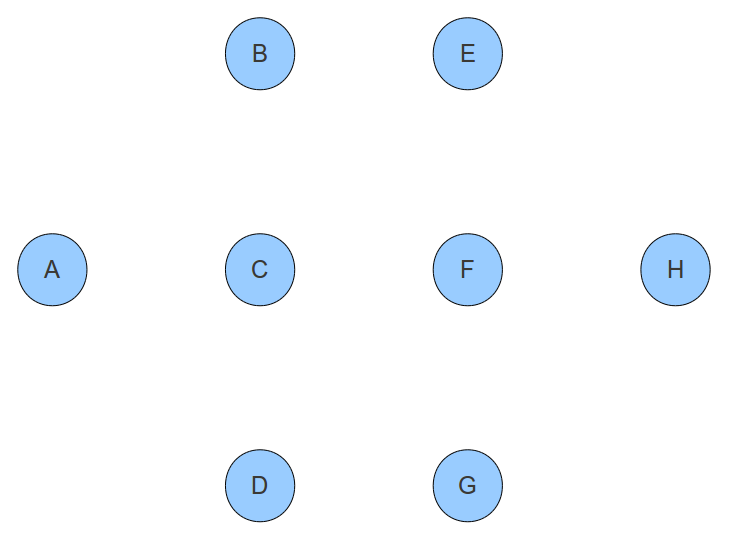
\includegraphics[width=0.5\textwidth]{../doc/img/exemplo1/passo5.png}
\caption{$C=\{A, E, F, G\}$}
\label{fig:exemplo1-passo5}
\end{figure}
}

\frame{
\frametitle{Resposta final}
\begin{figure}[ht]
\centering
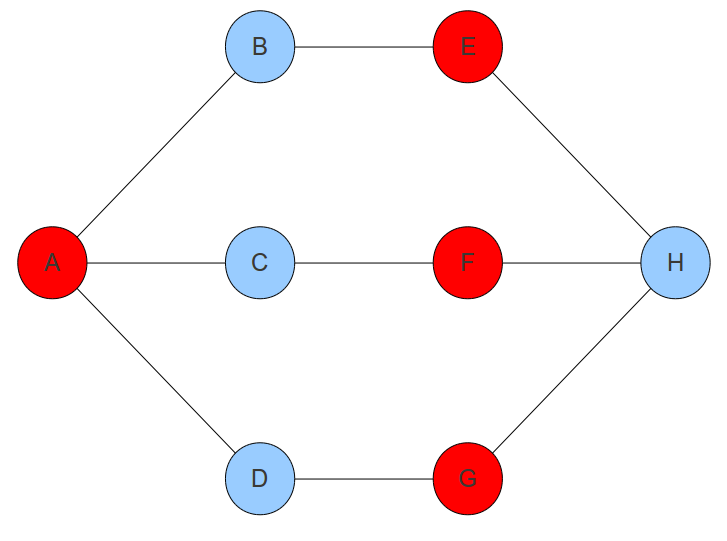
\includegraphics[width=0.5\textwidth]{../doc/img/exemplo1/final.png}
\caption{Resposta final}
\label{fig:exemplo1-final}
\end{figure}
}

\section{Experimentos}
\frame{
\frametitle{Tipos de experimentos}
Serão realizados dois tipos de experimentos para validar o algoritmo:
\begin{description}
    \item[Qualidade] Experimentos realizados com o intuito de ver a
        diferença no tamanho da CMV do grafo, e da CV encontrada
        pelo algoritmo.
    \item[Eficiência] Experimentos realizados com o intuito de
    averiguar o quão rápido o algoritmo realmente é.
\end{description}
}
\subsection{Qualidade}
\frame{
\begin{itemize}
    \item Foram usados 20 grafos da literatura como entrada para
    algoritmo, a fim de ter uma ideia da qualidade das CMVs geradas.
    \item Para cada grafo, serão apresentados três valores:
    \begin{description}
        \item[$n$] O número de vértices do grafo.
        \item[$k$] O tamanho da CMV.
        \item[$k'$] O tamanho da CV encontrada.
    \end{description}
\end{itemize}
}

\frame{
\frametitle{Grafo de Petersen~\cite{cite:example-petersen}}

\begin{figure}[htb]
\centering
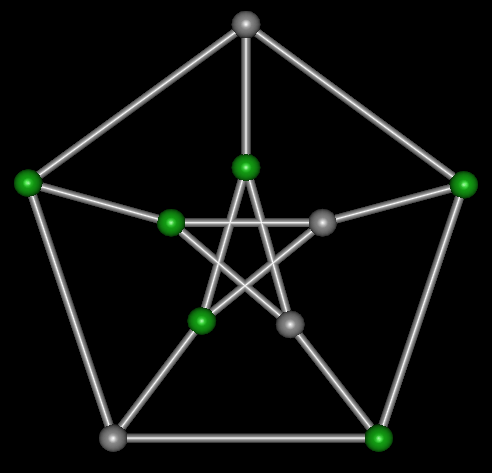
\includegraphics[width=0.5\textwidth]{../doc/img/petersen.png}
\caption{$n=10$, $k=6$, $k'=6$}
\label{fig:example-petersen}
\end{figure}
}

\frame{
\frametitle{Dodecaedro~\cite{cite:example-plato}}

\begin{figure}[htb]
\centering
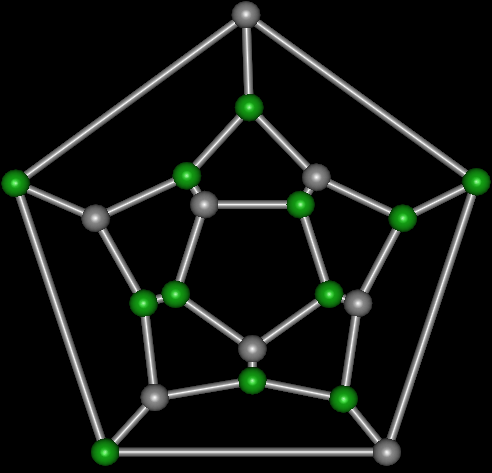
\includegraphics[width=0.5\textwidth]{../doc/img/dodecaedro.png}
\caption{$n=20$, $k=12$, $k'=12$}
\label{fig:example-dodecaedro}
\end{figure}
}

\frame{
\frametitle{Grafo de Berge~\cite{cite:example-berge}}

\begin{figure}[htb]
\centering
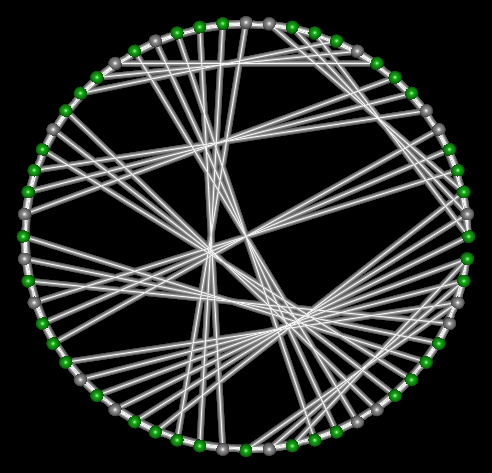
\includegraphics[width=0.5\textwidth]{../doc/img/berge.png}
\caption{$n=60$, $k=40$, $k'=40$}
\label{fig:example-berge}
\end{figure}
}

\frame{
\frametitle{Grafo de Bondy-Murphy $G_3$~\cite{cite:example-bondy}}

\begin{figure}[htb]
\centering
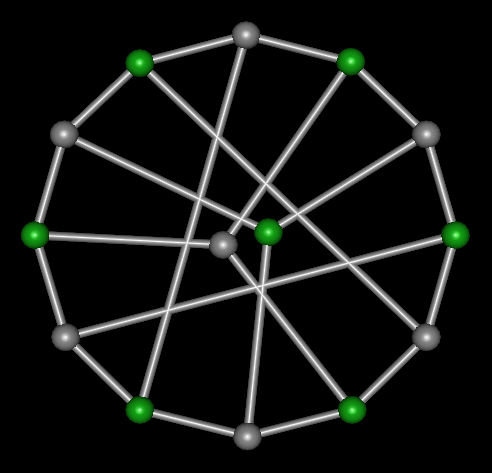
\includegraphics[width=0.5\textwidth]{../doc/img/bondymurphyg3.png}
\caption{$n=14$, $k=7$, $k'=8$}
\label{fig:example-bondymurphyg3}
\end{figure}
}

\frame{
\frametitle{Grafo de Witzel~\cite{cite:example-witzel}}

\begin{figure}[htb]
\centering
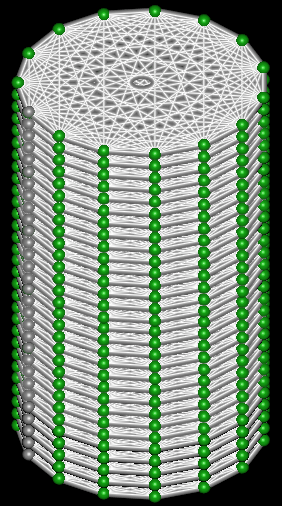
\includegraphics[height=0.7\textheight]{../doc/img/witzel.png}
\caption{Grafo de Witzel, $n=450$, $k=420$, $k'=429$}
\label{fig:example-witzel}
\end{figure}
}

\subsection{Eficiência}
\frame{
\frametitle{Preparativos}
\begin{itemize}
    \item Será usado o \textit{Python Web Graph
        Generator}~\cite{cite:pythonwebgenerator} para a geração de
        grafos aleatórios com número determinado de vértices e
        arestas.

    \item Foram executados alguns testes em uma máquina Linux, com
        processador Intel Core 2 Duo T8100, de 2.10GHz e 3GB de
        memória principal.

    \item Qual a melhor estratégia para definir o tamanho dos grafos
    de testes em termos de vértices e arestas?
\end{itemize}
}

\frame{
\frametitle{Alguns dados}
\begin{table}
\centering
\begin{tabular}{|c|c|c|}
\hline
\textbf{Tamanho} & \textbf{Tempo (s)} \\
\hline
$V=100, E=3000$ & 0.021 \\
\hline
$V=200, E=12000$ & 0.037 \\
\hline
$V=500, E=75000$ & 0.152 \\
\hline
$V=1000, E=300000$ & 0.546 \\
\hline
\end{tabular}
\caption{Alguns dados experimentais}
\end{table}
}

\section{Comentários finais}
\frame{
\frametitle{Comentários finais}

\begin{itemize}
    \item Não encontramos uma heurística similar na literatura.
    \item As respostas dadas pela heurística são bastante próximas do
    ótimo.
    \item Apesar do tempo $O(VE)$, o algoritmo parece executar
    bastante rápido. Pelo menos para os exemplos utilizados.
\end{itemize}


}

% =================== Bibliografia ==================== %
\appendix
\section*{\appendixname}
    \subsection*{Referências}

    \begin{frame}[allowframebreaks]
      \frametitle{Bibliografia}
        \nocite{*}
        \bibliographystyle{amsplain}
        \bibliography{../doc/tp.bib}

    \end{frame}
\end{document}
